\documentclass[UTF8]{ctexart}

\usepackage[linesnumbered,boxed,ruled,commentsnumbered]{algorithm2e}
\usepackage{bm}
\usepackage{graphicx}
\usepackage{float}
\usepackage[bookmarks=true]{hyperref}
\usepackage{amsmath}
\begin{document}
\title{基于深度学习的图像分类}
\author{陈昭熹 2017011552}
\maketitle
\tableofcontents
\newpage

\section{任务介绍}
任务要求完成10类图片的分类问题,数据格式为$28\times28$的灰度图片。本文将使用三种深度学习方法完成图像分类任务,本文后续内容将从模型搭建\ref{chapter:1}、训练方法及过程\ref{chapter:2}、模型调优\ref{chapter:3}以及最终的分类结果和评测\ref{chapter:4}来展开阐述。

\section{模型搭建}\label{chapter:1}
按照改进的先后顺序,分别采用全卷积神经网络,残差神经网络,Inception网络来实现图像分类任务。
\subsection{全卷积神经网络}
本节使用由四层卷积构成的全卷积神经网络,输出端由全连接层映射到分类类别,具体网络结构如下所示:
\begin{figure}[H]
    \centering
    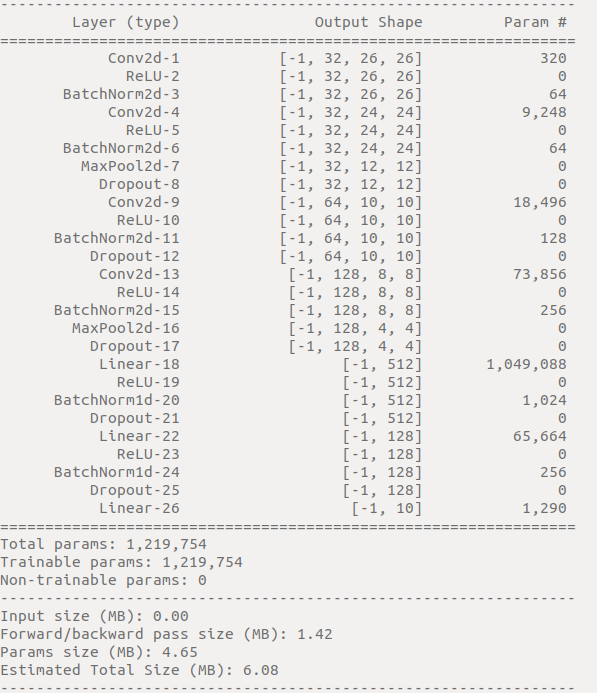
\includegraphics[scale=0.4]{../images/cnn4.png}
    \caption{四层全卷积网络}
\end{figure}
由于图像较小,故仅使用了两个最大池化来减少参数数量,并提取高级特征。

\subsection{残差神经网络}
本节使用基于BasicBlock的Resnet18完成图像分类任务。

在实验过程中,前一节所使用的四层全卷积结构出现了表达能力不足的情形,其参数量过少,难以区分一些高难度样本,不能很好的提取出高级特征。简单的增加网络层数可以提高神经网络的表达能力,但是本次任务数据量有限,且图像尺寸有限,盲目增加网络层数会出现\textbf{梯度退化}的问题,导致梯度反向传播无法更新到全网络,使得训练难以进行。Resnet的提出旨在解决深度神经网络难以训练的问题,将对直接特征的学习,通过shortcut的建立转变为对残差的学习,这使得梯度的反向传播能够顺畅抵达任意一层网络,使得学习变得更加容易,也让深层网络的训练成为可能,避免了层数增加准确率反而降低的问题。本节使用BasicBlock作为基础模块,而非BottleNeck结构。一个典型的BasicBlock结构如下:
\begin{figure}[H]
    \centering
    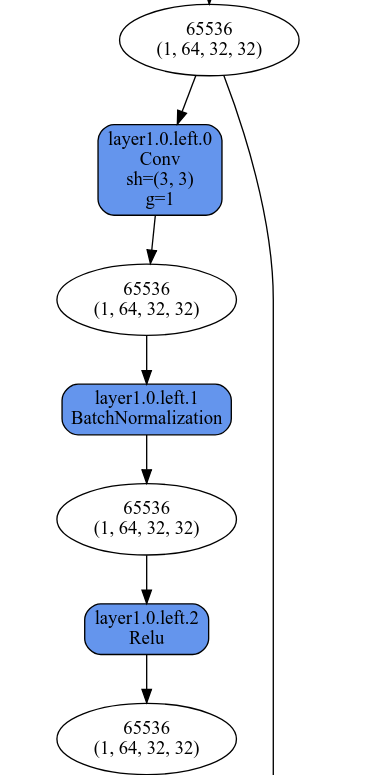
\includegraphics[scale=0.3]{../images/resblock1.png}\\
    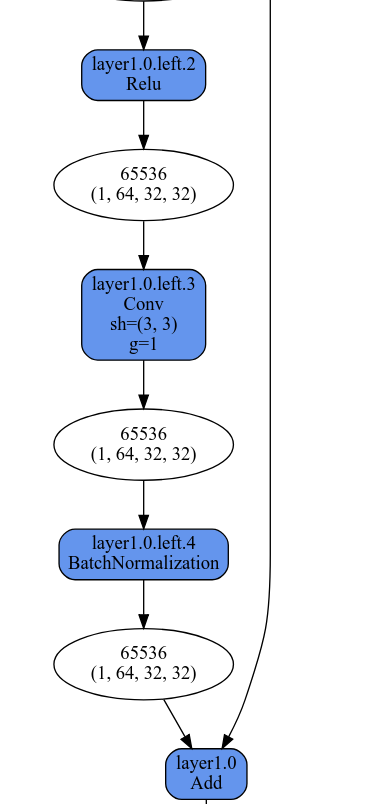
\includegraphics[scale=0.3]{../images/resblock2.png}
    \caption{残差网络中的BasicBlock}
\end{figure}

注意到输出层的全连接进行了升维再降维的处理,最终分类器映射到分类类别10.

\subsection{Inception模块}

本节使用基于Googlenet中的Inception模块搭建的网络完成图像分类任务。

由于图像尺寸有限,在进行多次卷积或池化后可能会导致后面的隐藏层很难再从中提取到有用的特征,因此在浅层就应当将图像中的各种类型特征尽可能提取出来输入到网络中。从这样的想法出发,本文采用GoogleNet中的Inception模块来在每一层中使用不同的卷积结构提取不同的特征,保证了数据的充分利用,提高网络泛化能力。一个Inception模块由$1\times1$,$3\times3$,$5\times5$以及$MaxPooling$构成,如下所示:
\begin{figure}[H]
    \centering
    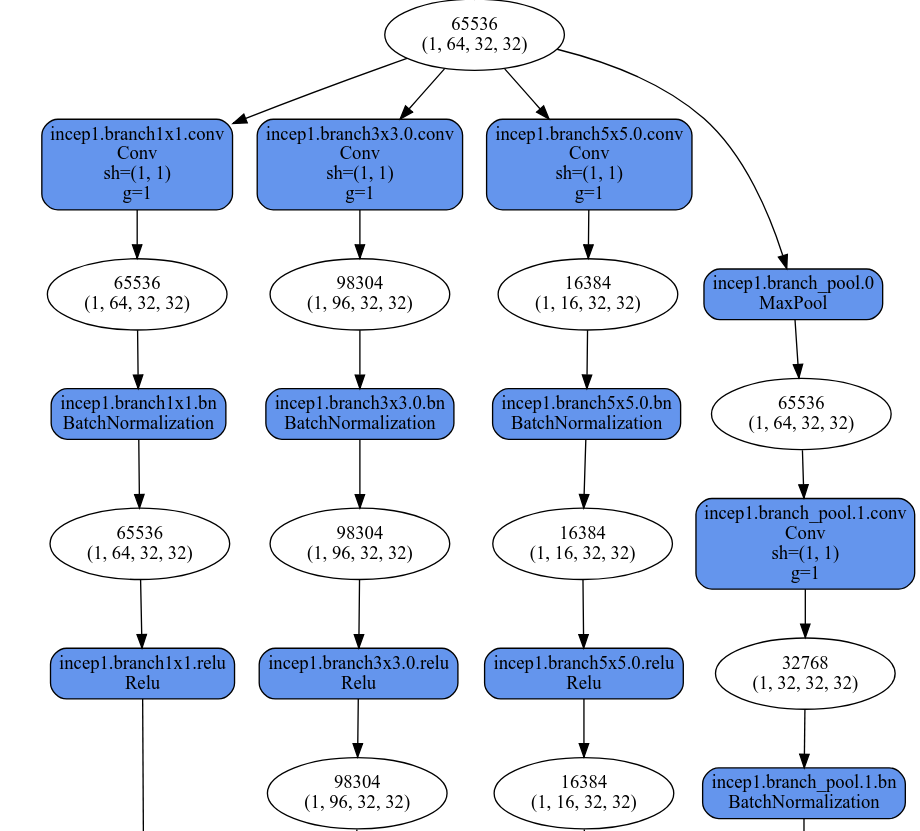
\includegraphics[scale=0.2]{../images/incepblock1.png}
    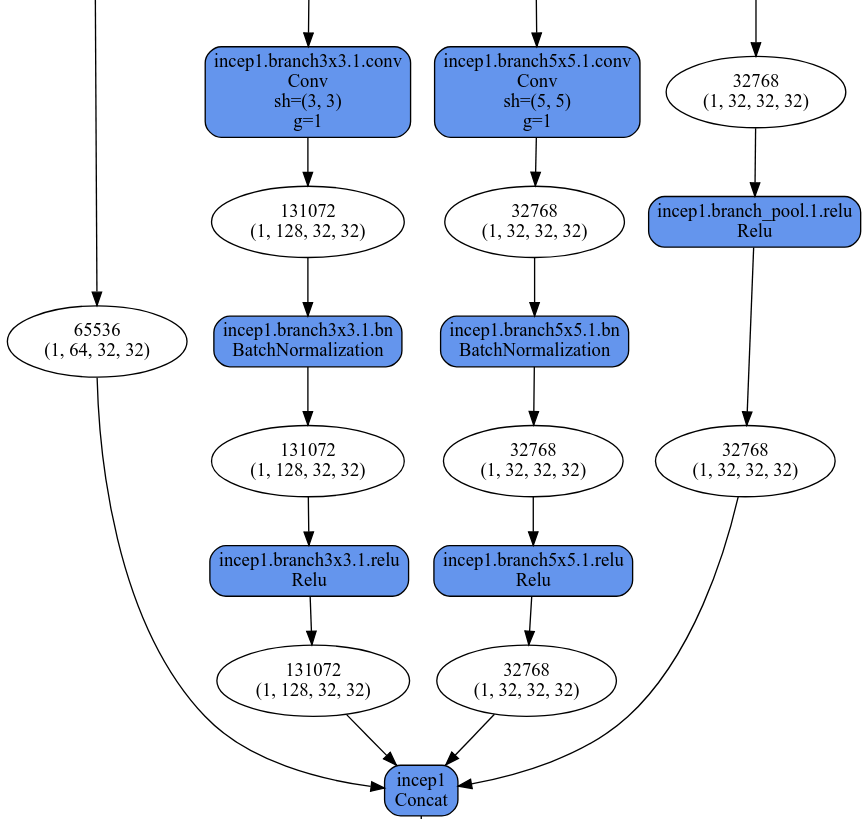
\includegraphics[scale=0.2]{../images/incepblock2.png}
    \caption{Inception模块}
\end{figure}
由多个这样的Inception模块堆积成网络,其层数较深这里就不做可视化了。


\section{训练方法及过程}\label{chapter:2}
\subsection{原始训练集处理}
为了保证训练过程及时终止,避免欠拟合和过拟合,将原始训练集的30000张图片,按照9:1的比例随机分成了训练集和验证集,即本地训练集包含10种类别,共27000张图像及其标签,本地验证集包含10种类别,共3000张图像及其标签。经过直方图统计,验证了划分出来的两个数据集中的类别分类近似均匀分布,不存在数据失衡问题。

\subsection{损失函数及优化器}
损失函数使用交叉熵,分类类别为10,定义如下:
\begin{equation}
    \text{loss}(x, class) = -\log\left(\frac{\exp(x[class])}{\sum_j \exp(x[j])}\right)
    = -x[class] + \log\left(\sum_j \exp(x[j])\right)
\end{equation}

优化器使用了两种,$SGD+Momentum$以及$Adam$,由于前者使用梯度的一阶矩估计,后者使用梯度的二阶矩估计,在不同情况下有不同的用途和表现。在下一章节中会阐述两种优化器在训练过程中的用途。

\subsection{Warm Up}
若使用复杂网络结构,参数量大,这使得学习率不宜过大,否则会错过最优解。另一方面考虑,由于数据量大,特别是在经过数据增广后,这使得学习率不能太小,否则训练效率会极低,网络训练时间会变长。为了平衡这两者,采用WarmUp策略,在正式训练之前,首先进行少量epoch的预训练,让网络参数有大概在最优解附近的取值,再进行正式训练。WarmUp使用Adam优化器,学习率设置为0.001,训练5个epoch后保存当前模型,便于开展后续的正式训练。

正式训练使用SGD+Momentum(0.9)优化器,由于Adam的优异性能,在预训练阶段模型基本上已经收敛到了最优解附近的范围内,此时使用SGD进行更为精确地求解,以保证能够最终找到最优解,避免了错过最优解或者陷入局部最优的情况。

\subsection{学习率Schedule}
随着网络层数加深,模型变得复杂,最优解点会变得越来越不稳定,优化器有时会很容易错过。这要求越到网络训练后期,优化器更新梯度的步长应当越小,保证能够收敛到极值点。由于Momentum的存在,不需要担心陷入局部最优的情形。基于这样的考量,本文在训练过程中采取动态改变学习率的策略,随着迭代的epoch数变大,逐步削减学习率。一个迭代200代的典型训练过程的学习率变化如下所示:
\begin{figure}[H]
    \centering
    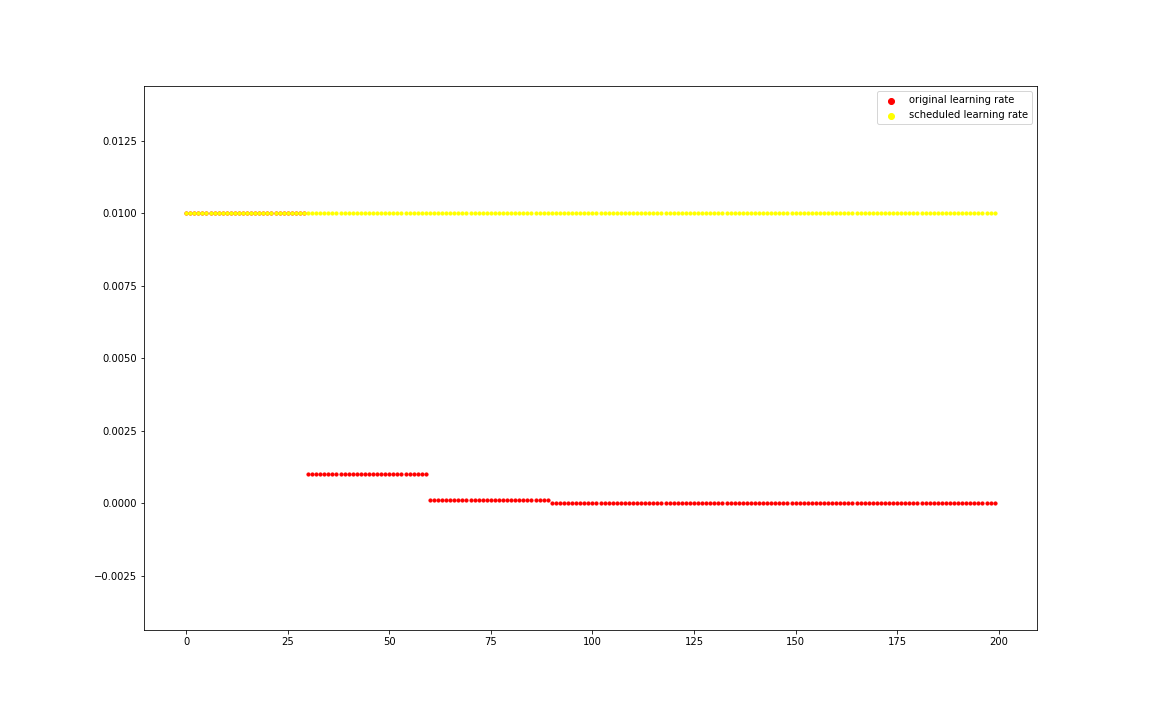
\includegraphics[scale=0.25]{../images/lrschedule.png}
    \caption{学习率Schedule}
\end{figure}



\section{调优}\label{chapter:3}
本文使用若干方法进行了调优,以获得更好的分类预测效果。
\subsection{Grid Search确定超参数}
在训练过程中,超参数包括$batch\_size,epoch\_num,learning\_rate$等,由于前文已述,学习率$learning\_rate$使用动态调整策略,因此能调节的超参数有$batch\_size,epoch\_num$,实验证明不同的批数量和迭代次数会对训练结果产生较大影响。
批数量$batch\_size$影响训练速度和梯度更新的平滑程度,较大的batch能够高效的利用GPU的并行计算能力,加快训练速度。而较小的batch能够针对性的将每一类的样本特征较好的进行反向传播,避免了细节特征被大量数据淹没。
迭代次数$epoch\_num$会影响网络的拟合效果,过少会导致欠拟合,不能发挥出网络实际的表达能力。过多会导致过拟合,降低网络的泛化能力,在测试集上表现会大幅下降。
为了确定哪种超参数组合最适合当前任务和当前的网络结构,保证超参数的设置能够表现出网络最佳的表达能力,为后续调优减少干扰因素,本文使用网格搜索方法(Grid Search)确定超参数组合,搜索空间如下:
\begin{equation}
    \begin{cases}
        batch\_size \in \{32,64,128,256,512\}\\
        epoch\_num \in \{20,30,40,50,60,70,80,90,100,200\}
    \end{cases}
\end{equation}

根据网络训练结果在验证集上的表现,确定最优超参数组合。
以全卷积神经网络结构为例,进行的Grid Search,以判据为验证集准确率,最终确定超参数组合为(64,80)。而结合了学习率Schedule后,epoch数这一项可以无需进行调节,在训练过程中设置checkpoint即可。


\subsection{批正则化}
为了解决梯度弥散问题,让网络更加易于训练,在每一层卷积后增加了BN层,调整每一层输出的数据的分布,保证了梯度的有效性。下面阐述Batch Normalization的原理,其本质就是将每一个batch的数据在每一层卷积后重新变换为均值为0方差为1的分布。首先求取batch均值和方差:
\begin{equation}
    \mu_B = \frac{1}{n}\sum^n_{i=1}x_i
\end{equation}
\begin{equation}
    \sigma_B^2 = \frac{1}{n}\sum^n_{i=1}(x_i-\mu_B)^2
\end{equation}

归一化:
\begin{equation}
    x_i'=\frac{x_i-\mu_B}{\sqrt{\sigma_B^2}}
\end{equation}

\subsection{DropOut}
Dropout使用基于概率的策略,将网络中某层的一部分参数随机丢弃,能够一定程度上防止过拟合发生,同时提高模型的泛化能力。事实上,在使用了批正则化后,网络中再加入DropOut的必要性还需要严格的论证。但对于上文提及的Resnet网络结构和Inception网络结构,其输出层的全连接采取了多层结构,也具有相当可观的参数量。经过实验,在输出层的全连接之间增加Dropout能够显著的降低过拟合的可能,并一定程度提高模型泛化能力。

\subsection{训练集处理}
\subsubsection{数据增广}
深度学习说到底还是一个data-driven的方法,因此如果能够有更多的、合适的数据,则一定会提高模型的拟合能力,让其在测试集上表现更好,是所谓见多识广。因此本文使用了在训练集上进行数据增广的方法来扩充训练样本。

值得注意的是,数据增广的方法需要避免生成的样本与原样本有过多的相似之处。若生成的训练样本与原样本过于相似,则会导致两个样本输入到网络中后,提取出的特征基本一致,强化了对单一样本的拟合,变相降低了泛化能力,相当于训练过程网络见到同一个样本两次。为了避免这一问题,本文采取水平翻转+随机擦除+高斯滤波的方法,将训练集扩充为原来的三倍大小,即新训练集中包含原训练集全部样本和水平翻转后进行随机擦除的训练样本以及原样本经过高斯滤波的训练样本。
\begin{figure}[H]
    \centering
    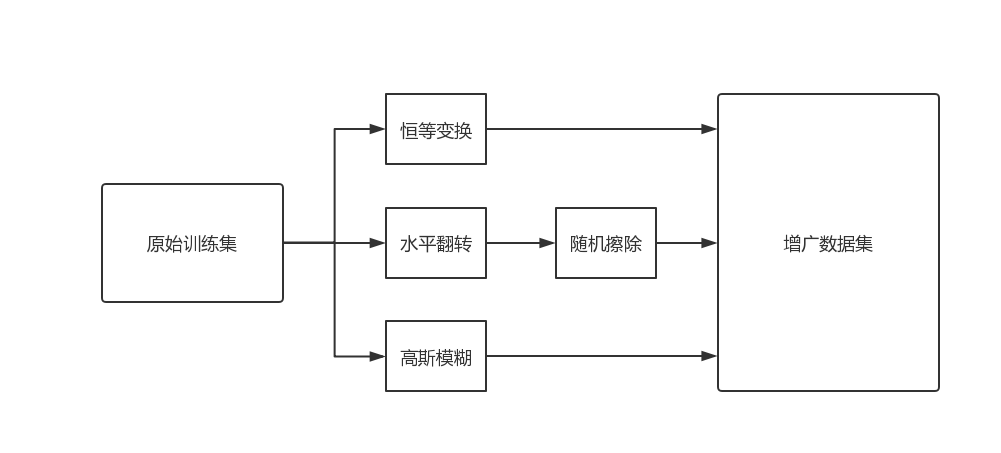
\includegraphics[scale=0.3]{../images/dataaug.png}
    \caption{数据增广流程}
\end{figure}
这种方法仅在训练全卷积神经网络使用,为了弥补其特征提取能力不足的短板。

\subsubsection{数据增强}

而对于残差网络和Inception网络,其深度保证了其特征提取能力是足够的。因此为提升泛化能力,只需要将原训练集的样本进行数据增强,让同一类别的样本尽可能不出现相似的pattern,进而提高分类性能。
本文采用的数据增强方法有:随机水平翻转、随机旋转、随机裁剪、随机擦除。


\subsection{多模型联合决策}

不同的网络结构拥有不同的特征提取和表达能力,同时训练过程的梯度更新的随机性也会导致每个模型训练出的效果有微小差别。为了融合不同模型的特征表达能力,提高最终预测时对于难分辨类别的分类能力,同时避免参数训练过程带来的方差的影响,本文采取多模型联合决策的策略,在生成测试集标签的过程中,使用多个模型的输出,通过加权平均来最终得到分类结果。

值得注意的是,每个网络的参数不同、结构不同,其输出层输出的10个值不一定具有可加性。但由于本次是一个分类任务,因此其概率分布是具有可加性的,因此在多模型联合决策的过程中,使用$softmax$将每个模型的输出转化为概率分布,利用概率的可加性进行加权平均,再取其中概率最大的标签作为最终的分类结果。

这样做的好处是,可以针对难以区分的特征专门训练强分类器,例如本次任务中标签为0和6的样本是难样本,标签为2和4的样本也难以区分。可以针对这种情况,对优化器设置梯度权重,增加难样本的梯度权重,从而使得网络更倾向于区分所设定的难样本,最终通过多模型联合决策来得到更好的分类效果。本文最终的结果为4模型联合决策,其中使用了一个基于Resnet训练的强分类器,其10个标签的梯度更新权重为:
\begin{equation}
    weights = [2.0,0.8,1.5,0.8,1.5,1.2,2.0,1.2,1,1.2]
\end{equation}

其中以Resnet为例,在不使用梯度带权更新时性能如下,可以与后面的强分类器性能作对比\ref{resnet},差别一目了然
\begin{figure}[H]
    \centering
    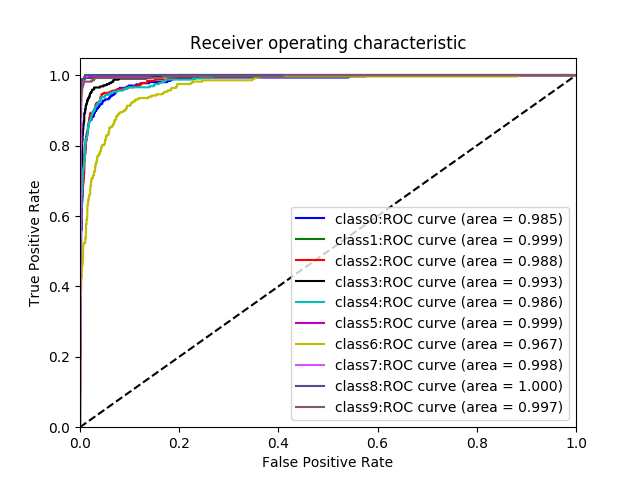
\includegraphics[scale=0.35]{../images/res18roc.png}
    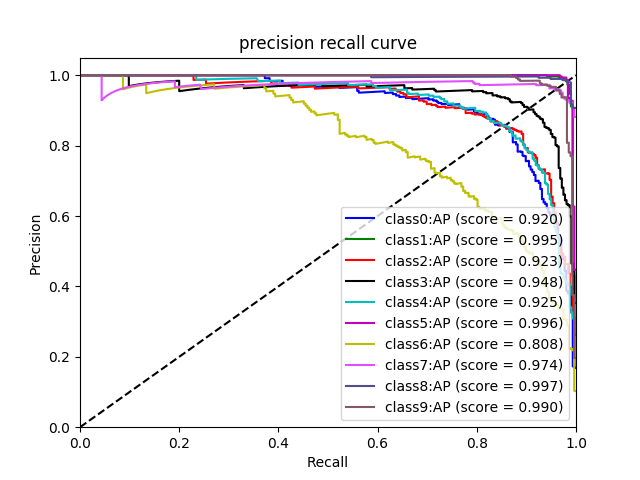
\includegraphics[scale=0.35]{../images/res18pro.png}
    \caption{残差网络——非强分类器}
\end{figure}

\section{实验结果与评测}\label{chapter:4}
本节以不同网络在验证集上的ROC图像和准确率召回率图像,以及最终在测试集上的准确率来评估结果。
\subsection{全卷积网络}
\begin{figure}[H]
    \centering
    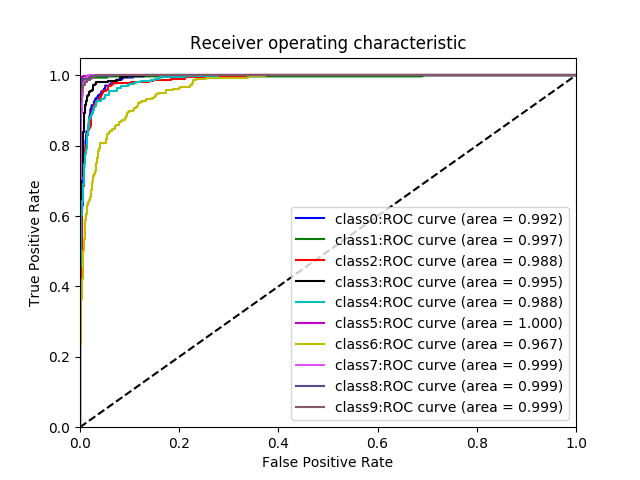
\includegraphics[scale=0.35]{../images/cnn4roc.png}  
    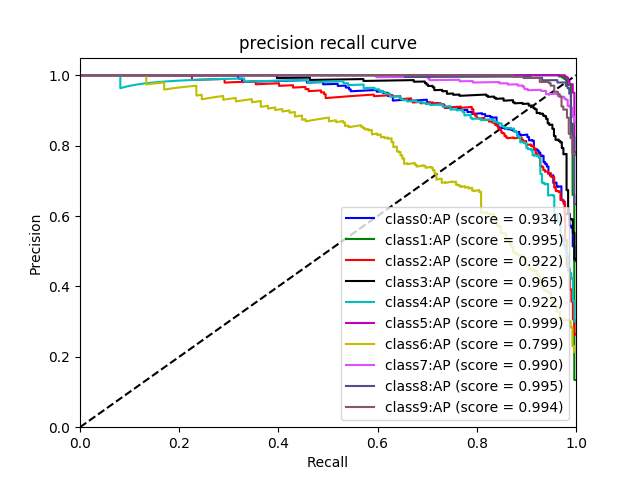
\includegraphics[scale=0.35]{../images/cnn4pro.png}
    \caption{全卷积网络}
\end{figure}


\subsection{残差网络}\label{resnet}
\begin{figure}[H]
    \centering
    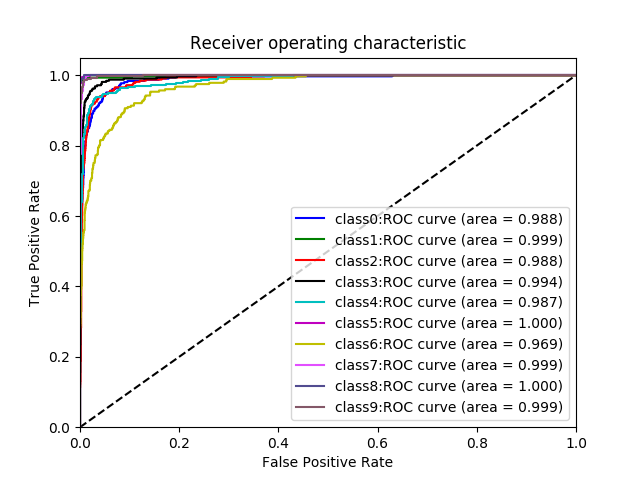
\includegraphics[scale=0.35]{../images/weightresroc.png}
    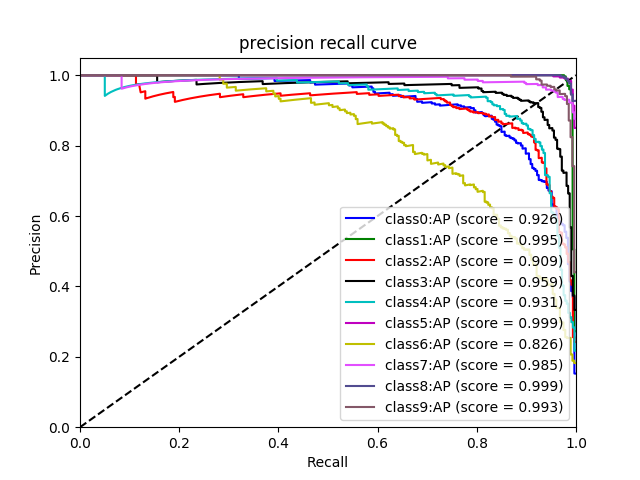
\includegraphics[scale=0.35]{../images/weightrespro.png}
    \caption{残差网络——强分类器}
\end{figure}

\subsection{Inception网络}

\begin{figure}[H]
    \centering
    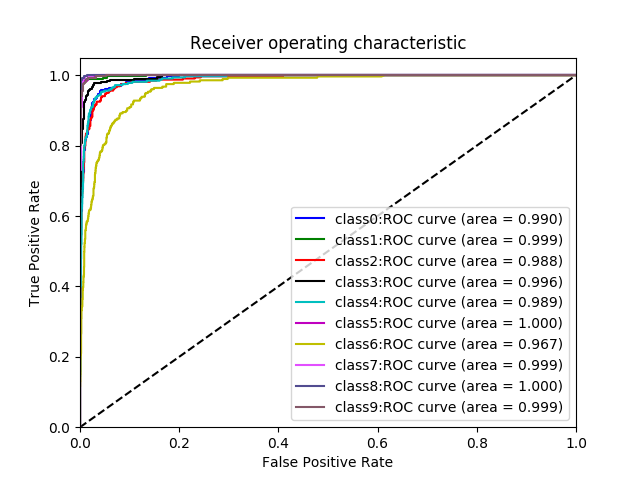
\includegraphics[scale=0.35]{../images/inceproc.png}
    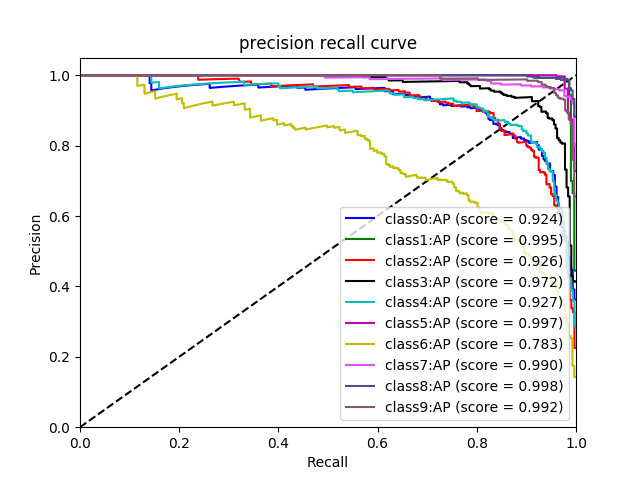
\includegraphics[scale=0.35]{../images/inceppro.png}
    \caption{Inception网络}
\end{figure}

最终获得的验证集以及测试集准确率如下,可以看出随着网络结构不断改进,以及模型融合策略的使用,准确率不断升高,达到了调优的目的。

\begin{table}[H]
\centering
\begin{tabular}{ccc}
    \hline
    模型& 验证集准确率& 测试集准确率(以Public榜为参考)\\
    \hline
    4-CNN & $89.63\%$ &$89.53\%$\\
    Resnet & $91.28\%$&$88.60\%$\\
    Inception &$90.97\%$ & $90.06\%$\\
    ModelFusion &$91.72\%$&$90.33\%$\\
    \hline
\end{tabular}
\end{table}

最终kaggle榜上情况如下:
\begin{table}[H]
    \centering
    \begin{tabular}{ccc}
        \hline
        队名(\textbf{FrozenBurning})&Public榜&\textbf{Private榜}\\
        \hline
        分数 & $90.333\%$ &$91.257\%$\\
        排名 &$55$ &$25$\\
        \hline
    \end{tabular}
\end{table}

\section{总结}

本次大作业,确实收获良多。在kaggle打榜的驱动力下,从零开始,从简单结构做起,一步步地改进网络结构,优化超参数,学习神经网络的工作机理和参数问题,最终较好的完成了图像分类任务。不同的网络结构、参数设置会导致不同的结果,在计算量、模型复杂度、模型性能、网络效率等多方面均需要进行考量,才能获得较满意的效果。

\end{document}